% Springer Nature journal article template (Version 3.1, December 2024)
% Compile with pdfLaTeX and BibTeX in a project containing sn-jnl.cls and
% sn-basic.bst from the official Springer Nature LaTeX template package.
\documentclass[pdflatex,sn-basic,Numbered]{sn-jnl}

\usepackage{graphicx}
\usepackage{amsmath,amssymb,amsfonts}
\usepackage{booktabs}
\usepackage{braket}
\usepackage{array}
\usepackage{tabularx}
\usepackage{enumitem}
\usepackage{xurl}

% PDF metadata; hyperref is loaded by the Springer Nature class.
\AtBeginDocument{\hypersetup{
  pdftitle={Factorial Benchmarking of Exact and Finite-Shot Gradient Resolvability in a Four-Qubit Hybrid Quantum Neural Network},
  pdfauthor={Brandon Shen},
  pdfsubject={Factorial benchmarking of exact-gradient signal and finite-shot resolvability in a four-qubit hybrid QNN},
  pdfkeywords={quantum machine learning, quantum neural networks, factorial design, finite-shot gradient estimation, gradient resolvability, reproducible benchmarking}
}}

\urlstyle{same}
\newcommand{\cx}[2]{CX($#1\!\to\!#2$)}
\newcommand{\snrstar}{\mathrm{SNR}^{*}_{\mathrm{est}}}
\newcommand{\snrest}{\widehat{\mathrm{SNR}}_{\mathrm{est}}}
\newcommand{\snrexact}{\mathrm{SNR}_{\mathrm{exact}}}
\newcommand{\vshots}{\mathrm{Var}_{\mathrm{shots}}}

\setlist{nosep,leftmargin=*}
\setlength{\emergencystretch}{1.5em}
\raggedbottom

\begin{document}


\title[Factorial Benchmarking of QNN Gradients]
{Factorial Benchmarking of Exact and Finite-Shot Gradient Resolvability in a Four-Qubit Hybrid Quantum Neural Network}

\author*[1]{\fnm{Brandon} \sur{Shen} (ORCID: \href{https://orcid.org/0009-0002-3545-2106}{0009-0002-3545-2106})} \email{brandonshen123@gmail.com}

\affil*[1]{\orgname{Independent Researcher},
\orgaddress{\city{Belmont},
\state{California}, \postcode{94002}, \country{United States}}}

\abstract{\textbf{Purpose:} We evaluate whether circuit, objective, and hybrid-connectivity interventions combine non-additively in exact-gradient signal and finite-shot resolvability for a four-qubit quantum neural network.

\textbf{Methods:} A complete $2^3$ factorial benchmark crossed a pair-restricted CNOT schedule, normalized transverse-field Ising energy objective, and fixed residual shortcut in a measure--re-encode--reset architecture. Centered binary coding made lower-order interactions equal averages over the third factor. The frozen study used 50 matched initialization clusters and 30 finite-shot replicates per scientific cell, with configurations matched by block count, parameter identity, and total implemented simulator-shot budget.

\textbf{Results:} The exact-gradient $E\times L$ interaction was supported by both model-based inference and initialization-cluster bootstrap. Its positive direction was retained in a new-seed dataset, although magnitude, depth profile, covariance dependence, and weighting dependence remained uncertain. Finite-shot $E\times L$ and $E\times R$ interactions met the protocol-derived Wald/Holm rule, but their 443-completed-fit nested-bootstrap intervals included zero. The residual-related result was objective-specific, estimator-mode sensitive, and inactive by construction at $D=1,2$; the $L\times R$-by-depth interaction remained unresolved.

\textbf{Conclusion:} Factorial benchmarking separates exact signal from finite-shot measurement behavior and exposes inference-dependent composition effects. These initialization-gradient results do not establish optimization success, trainability improvement, hardware advantage, shot savings, or matched physical-resource cost.}

\keywords{quantum machine learning, quantum neural networks, factorial design, finite-shot gradient estimation, gradient resolvability, reproducible benchmarking}

\maketitle

\section{Introduction}\label{sec:introduction}

Variational quantum algorithms and quantum neural networks (QNNs) optimize parameterized circuits through expectation values or their derivatives \cite{cerezo2021vqa,mitarai2018quantum,schuld2019evaluating}. Their practical behavior depends jointly on circuit structure, objective construction, initialization, optimization, and measurement. Barren plateaus are one important failure mode, but the absence of asymptotically vanishing gradients does not guarantee that a finite-shot optimizer receives a reliable update direction \cite{mcclean2018barren,anschuetz2022traps,thanasilp2023subtleties,larocca2025barren}. This study therefore asks a narrower operational question: whether a gradient component is resolvable under a specified finite-shot protocol.

Prior work has examined local objectives, restricted entanglement, structured initialization, hybrid architectures, and residual connections largely in separate models and against separate baselines \cite{cerezo2021costfunction,ortizmarrero2021entanglement,patti2021entanglement,grant2019identity,skolik2021layerwise,beer2020training,kashif2024resqnets}. Finite-shot studies likewise show that gradient precision and acquisition cost depend on the observable, circuit, and measurement allocation \cite{kubler2020adaptive,tamiya2022stochastic,kreplin2024finite,chinzei2025tradeoff,bowles2025backpropagation}. These results establish important marginal effects, but they do not determine whether interventions reinforce, cancel, or otherwise modify one another when combined.

A complete factorial design estimates such composition effects directly \cite{montgomery2019design}. We cross three interventions that act at different points in a hybrid computation: a pair-restricted within-block CNOT schedule ($E$), normalized TFIM energy in place of global target-state infidelity ($L$), and a fixed-gain classical residual shortcut between independently reset blocks ($R$). The experiment holds initialization seeds, matched quantum parameters, block counts, and total shot budgets fixed across all eight configurations.

The study follows the factors, hypotheses, model families, transformations, and multiplicity procedure described in a previously published protocol article \cite{shen2026gradient}. That article proposed the factorial experiment and reported no data or results from the implementation analyzed here. It did not constitute a complete preregistration: reset semantics, residual activation, plug-in-SNR eligibility, estimator-mode enforcement, and several robustness procedures were resolved during implementation or added after the primary outputs were inspected. We therefore describe H1--H4 as \emph{protocol-derived primary analyses conditional on the reset-per-block implementation}, not as unconditional preregistered tests, and label every later validation, sensitivity, and independent-seed analysis explicitly.

The contribution is threefold. First, the experiment directly estimates non-additive effects among three QNN gradient-resolvability strategies under matched conditions. Second, it separates exact-gradient magnitude, finite-shot resolvability, estimator bias, sign reliability, task metrics, and measurement cost rather than collapsing them into a single claim of ``trainability.'' Third, it provides an audited and reproducible implementation with deterministic seeds, black-box gradient validation, guarded estimator-mode separation, frozen outputs, and regression tests. The primary empirical result is a positive $E\times L$ exact-gradient interaction supported by both model-based and resampling analyses. The finite-shot analogue is presented as qualified evidence because it is conditional on estimator eligibility and sensitive to inference method and block count.

\section{Background and study questions}

\subsection{Finite-sample gradient usability}

For parameter $\theta_k$, let $\hat g_{kr}(\theta)$ be replicate $r$ of the complete finite-shot gradient estimator, $\mu_k=\mathbb{E}_{\mathrm{shots}}[\hat g_{kr}\mid\theta]$, and $\sigma_k^2=\mathrm{Var}_{\mathrm{shots}}[\hat g_{kr}\mid\theta]$. The inaccessible repeated-shot population target is
\[
\snrstar_k=\frac{|\mu_k|}{\sigma_k}.
\]
With $R_{\mathrm{rep}}=30$ independent finite-shot replicates, the analyzed plug-in estimator is
\[
\snrest_k=\frac{|\bar g_k|}{s_k},\qquad
\bar g_k=\frac{1}{30}\sum_{r=1}^{30}\hat g_{kr},\qquad
s_k^2=\frac{1}{29}\sum_{r=1}^{30}(\hat g_{kr}-\bar g_k)^2.
\]
When an exact statevector derivative is available, the complementary measure is
\[
\snrexact(\theta)=
\frac{|g_k^{\mathrm{exact}}(\theta)|}{s_k},
\qquad
\mathrm{Bias}_k(\theta)=\mu_k(\theta)-g_k^{\mathrm{exact}}(\theta).
\]
High $\snrest$ indicates that the estimator's own mean is distinguishable from its repeated-shot uncertainty. It does not establish unbiasedness, correct sign, convergence, or task fidelity, so these outcomes are reported separately.

H2--H4 analyze $\snrest_k$, not $\snrstar_k$. The plug-in ratio carries finite-replicate uncertainty, motivating resampling of both initialization clusters and within-cell replicates. It is undefined when $s_k^2=0$; primary models exclude those cells without an epsilon or floor, and a labeled sensitivity assigns zero only when both $\bar g_k=0$ and $s_k^2=0$. Input validation rejects duplicate replicate keys and invalid rows before aggregation; the frozen production validation found neither. Online Resource~1 reports exclusions and conventions in detail.

\subsection{Interventions and interaction hypotheses}

The pair-restricted CNOT factor ($E$) changes the within-block schedule while holding the number of rotations and logical CNOT gates fixed. The objective factor ($L$) replaces global infidelity with normalized TFIM energy; it is a full objective contrast that changes spectral weighting, observable decomposition, measurement requirements, and landscape geometry, not a pure locality intervention. The residual factor ($R$) is a fixed-gain classical shortcut between independently reset quantum blocks and adds no quantum gates or observables.

The novelty claim is intentionally narrow: the individual interventions and metrics are established. To our knowledge, these three implemented contrasts have not previously been evaluated together in a matched factorial experiment that separates exact-gradient magnitude from finite-shot estimator behavior. The strongest prior expectation concerned $E\times L$, because the entangling schedule changes reduced-state derivatives while the objective selects and weights the derivative components entering the measured signal. The published protocol expected sub-additivity at the exact-signal level, but all tests are two-sided \cite{shen2026gradient}.

H1--H4 form one Holm-corrected family at family-wise $\alpha=0.05$:
\begin{itemize}
\item \textbf{H1:} the $E\times L$ coefficient $\eta_{EL}$ in $\operatorname{asinh}(|g^{\mathrm{exact}}|)$ differs from zero;
\item \textbf{H2:} the $E\times L$ coefficient $\beta_{EL}$ in end-to-end $\operatorname{asinh}(\snrest)$ differs from zero;
\item \textbf{H3:} the $E\times R$ coefficient $\beta_{ER}$ differs from zero;
\item \textbf{H4:} the block-count-moderated $L\times R$ coefficient $\beta_{LRD}$ differs from zero.
\end{itemize}
Depth-moderation analyses beyond H4, conditional-estimator analyses, active-residual subset analyses, and configuration-level comparisons are diagnostic or exploratory.

\section{Evaluation protocol and experimental setup}\label{sec:methods}
\subsection{Reference task and objectives}

The reference task is ground-state preparation for the four-site, open-boundary TFIM,
\[
H=-J\sum_{i=0}^{2}Z_i Z_{i+1}-h\sum_{i=0}^{3}X_i,
\qquad J=1,\quad h=0.5.
\]
The target ground state $\ket{\psi_0}$ and eigenvalue bounds $E_0\approx-3.4270$ and $E_{\max}\approx3.4270$ are obtained by exact diagonalization of the $16\times16$ Hamiltonian matrix. Let $\rho_0=\ket{\psi_0}\!\bra{\psi_0}$ and let $\rho(\theta)$ be the prepared state. The global objective is target-state infidelity,
\[
C_{\mathrm{global}}(\theta)
=1-\mathrm{Tr}[\rho_0\rho(\theta)],
\]
and the local objective is normalized TFIM energy,
\[
C_{\mathrm{local}}(\theta)
=\frac{\mathrm{Tr}[H\rho(\theta)]-E_0}{E_{\max}-E_0}.
\]
Both objectives have the same nondegenerate target ground state, preventing target identity from confounding the comparison. The resulting factor still represents the full contrast between normalized TFIM energy and global infidelity, not measurement locality alone: the objectives also differ in spectral weighting, observable decomposition, measurement requirements, and landscape geometry. Prepared-state energy and target fidelity at initialization are therefore reported for every configuration. These are terminal-block prepared-state metrics, not trained or optimized performance.

\subsection{Hybrid block architecture and entangling schedules}
\label{sec:ansatz}

To avoid conflict with the objective factor $L$, the number of hybrid blocks is denoted by $D\in\{1,2,3,4,6\}$. Each block applies one independently parameterized $R_y$ rotation to each qubit, followed by exactly four logical CNOT gates. $D$ is a \emph{hybrid block count}, not the depth of one continuously evolving quantum state: each block begins from $\lvert0000\rangle$, is evaluated and measured independently, and passes only classically re-encoded features to later blocks. The results therefore apply specifically to this measure--re-encode--reset architecture.

Every $x^{(\ell)},z^{(\ell)},\theta^{(\ell)}\in\mathbb{R}^{4}$; each $W_\ell\in\mathbb{R}^{4\times4}$ and $b_\ell\in\mathbb{R}^{4}$. The first input is $x^{(1)}=0$. In block $\ell$, qubit $q$ receives the angle $a_q^{(\ell)}=\theta_q^{(\ell)}+x_q^{(\ell)}$ in a single $R_y(a_q^{(\ell)})$ gate, followed by the four ordered CNOTs below. No clipping, modular wrapping, normalization, nonlinear activation, rescaling, or additional encoding gate is applied. For $\ell<D$, one shared computational-basis measurement yields $z_j^{(\ell)}=\langle Z_j\rangle$ for all four qubits; the register is then discarded. The terminal state is evaluated directly with the selected objective rather than converted to an inter-block $z^{(D)}$.

\begin{figure*}[t]
\centering
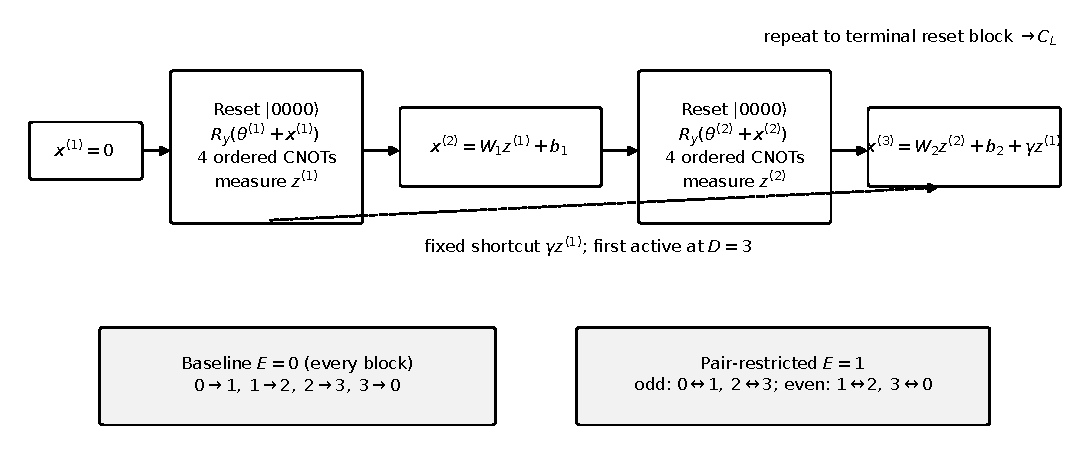
\includegraphics[width=.94\textwidth]{figures/fig16_architecture.pdf}
\caption{Implemented forward pass. Each quantum block starts from a reset four-qubit register, angle-encodes the four-dimensional classical feature by addition to four trainable $R_y$ angles, applies one of the two four-CNOT schedules, and either returns four $Z$ expectations to the classical transition or evaluates the terminal objective. The dashed shortcut is present only for $R=1$ and first changes $x^{(3)}$, so it is inactive for $D=1,2$. The baseline schedule is the ordered ring \cx{0}{1}, \cx{1}{2}, \cx{2}{3}, \cx{3}{0}; the pair-restricted schedule uses the ordered odd/even block pairings stated in the text.}
\label{fig:architecture}
\end{figure*}

Two logical CNOT schedules are used within each block:

\begin{itemize}
\item \textbf{Baseline ($E=0$):} \cx{0}{1}, \cx{1}{2}, \cx{2}{3}, \cx{3}{0}, in that order. The sequential schedule contains a causal path spanning the register within the block.
\item \textbf{Restricted ($E=1$):} odd-position blocks use \cx{0}{1}, \cx{2}{3}, \cx{1}{0}, \cx{3}{2}; even-position blocks use \cx{1}{2}, \cx{3}{0}, \cx{2}{1}, \cx{0}{3}. Each block acts within two disjoint pairs, with the pairing alternating by block position.
\end{itemize}

Both schedules are applied literally, gate by gate, in the statevector simulator, with no transpiler-level fusion or reordering. Because no quantum state persists across blocks, alternating the restricted schedule changes the paired qubits at each block position but does not accumulate entanglement across $D$ in the manner of alternating layers in one continuous circuit. Entanglement entropy and reduced-state purity are used only as finite-system diagnostics; no area-law or asymptotic scaling claim is made from four qubits.

\subsection{Residual hybrid architecture}
\label{sec:residual-arch}

For block $\ell\in\{1,\ldots,D\}$, the quantum node is
\[
z_j^{(\ell)}
=\mathrm{Tr}\!\left[Z_j\rho_\ell
  \!\left(x^{(\ell)},\theta^{(\ell)}\right)\right],
\qquad j=0,\ldots,3.
\]
The block is initialized from $\ket{0\ldots0}$ and depends only on its own encoded input $x^{(\ell)}$ and gate angles $\theta^{(\ell)}$. For $\ell=1,\ldots,D-1$, the next input is
\[
x^{(\ell+1)}=
\begin{cases}
W_\ell z^{(\ell)}+b_\ell+\gamma z^{(\ell-1)}, & R=1,\\[3pt]
W_\ell z^{(\ell)}+b_\ell, & R=0,
\end{cases}
\]
with fixed shortcut gain $\gamma=1$ in the residual condition and $\gamma=0$ otherwise. $W_\ell$ and $b_\ell$ are parameterized and initialized identically across residual and non-residual conditions; the fixed shortcut adds no trainable parameters, quantum gates, or additional observables.

For every initialization--$D$ pair, the code derives separate SHA-256-based seeds from root seed 20260726 for quantum and classical parameters. Each component of every $\theta^{(\ell)}$ is drawn independently from $\mathrm{Uniform}(0,2\pi)$. Each $W_\ell$ uses Glorot uniform initialization, $\mathrm{Uniform}[-\sqrt{6/(4+4)},\sqrt{6/(4+4)}]$, and $b_\ell=0$. All eight configurations at fixed initialization and $D$ reuse these same arrays and parameter indices; configurations are matched, not independently initialized. Different tested values of $D$ use independently derived depth-specific seeds, so deeper architectures do not reuse shallow prefixes. Shot streams are separately derived by initialization, $D$, configuration, estimator mode, $B$, and replicate.

One complete exact forward pass is therefore: initialize $x^{(1)}=0$ and $z^{(0)}=0$; for $\ell=1,\ldots,D$, reset the register, apply $R_y(\theta^{(\ell)}+x^{(\ell)})$ qubitwise and the ordered CNOT schedule; if $\ell<D$, measure $z^{(\ell)}$ and set $x^{(\ell+1)}=W_\ell z^{(\ell)}+b_\ell+\gamma z^{(\ell-1)}$; otherwise evaluate $C_L$ on the terminal state and return it.

The boundary convention is $z^{(0)}=0$. Therefore, the shortcut first changes a real block input at $x^{(3)}=W_2z^{(2)}+b_2+\gamma z^{(1)}$, which exists only when $D\ge3$. Thus, under matched seeds, $R=0$ and $R=1$ are structurally identical at $D\in\{1,2\}$ and diverge only from $D=3$ onward.

This activation threshold was identified during the post-run implementation audit and was not specified in the published protocol article's H3/H4 analysis \cite{shen2026gradient}. It therefore does not retroactively redefine the protocol-derived target population. The original full-sweep models remain the primary analyses conditional on the reset-per-block implementation. A $D\ge3$ active-residual analysis is reported as a sensitivity analysis, and the exact zero residual contrast at $D\in\{1,2\}$ is reported as a structural-validity check.

\subsection{Gradient assembly and validation target}

The terminal block's gradient is a direct parameter-shift derivative of the final cost. Every upstream total derivative is assembled by reverse-mode chain rule through the classical maps and quantum-node Jacobians,
\[
\frac{dC}{d\theta_k^{(\ell)}}
=\sum_j
\frac{\partial C}{\partial z_j^{(\ell)}}
\frac{\partial z_j^{(\ell)}}{\partial\theta_k^{(\ell)}}.
\]
Node-level derivatives are evaluated by the two-term parameter-shift rule for Pauli-generated rotations \cite{mitarai2018quantum,schuld2019evaluating}; the downstream sensitivities are propagated exactly through the classical maps. Classical gradients with respect to $W_\ell$ and $b_\ell$ are analyzed separately and are not pooled into the matched quantum-gradient distribution.

The finite-difference audit treats the complete hybrid cost as a black box and compares central finite differences against the assembled total derivative. The audit design is described here; numerical outcomes are summarized in Section~\ref{sec:results-robustness}, with full details in Online Resource 1.

\subsection{Complete factorial design}

All eight binary combinations of $E$, $L$, and $R$ are run (Table~\ref{tab:configurations}).

\begin{table*}[t]
\centering
\begin{tabular}{cccc l}
\toprule
\# & $E$ & $L$ & $R$ & Description \\
\midrule
1 & 0 & 0 & 0 & Baseline \\
2 & 1 & 0 & 0 & Pair-restricted CNOT schedule only \\
3 & 0 & 1 & 0 & TFIM-energy objective only \\
4 & 0 & 0 & 1 & Residual only \\
5 & 1 & 1 & 0 & $E+L$ combination \\
6 & 1 & 0 & 1 & $E+R$ combination \\
7 & 0 & 1 & 1 & $L+R$ combination \\
8 & 1 & 1 & 1 & All three interventions \\
\bottomrule
\end{tabular}
\caption{Complete $2^3$ factorial design}
\label{tab:configurations}
\end{table*}

Within each hybrid block count, all configurations share initialization seeds, matched quantum-gate parameter indices, and the same nominal shot-budget levels. The matched gradient distribution contains the $4D$ quantum rotation derivatives $dC/d\theta_q^{(\ell)}$ for $q=0,\ldots,3$ and $\ell=1,\ldots,D$. Derivatives with respect to the $16(D-1)$ entries of $W_\ell$ and $4(D-1)$ entries of $b_\ell$ are excluded from H1--H4 and are retained only in repository-level implementation outputs; the manuscript makes no substantive classical-gradient claim.

\subsection{Finite-shot estimator modes}

Two finite-shot modes are collected and reported separately:

\begin{itemize}
\item \textbf{End-to-end mode, primary for H2--H4:} forward features and node-level shifted measurements are independently re-estimated in every replicate. Nonlinear downstream re-encoding can therefore induce finite-shot estimator bias.
\item \textbf{Conditional mode, diagnostic:} forward features are held at their exact statevector values while node-level shifted measurements are resampled. This isolates Jacobian-estimation noise from uncertainty caused by re-estimating and re-encoding intermediate features.
\end{itemize}

The conditional mode is not a second primary test and cannot replace an unfavorable end-to-end result. Material disagreement between the modes is interpreted as sensitivity to forward-feature sampling rather than resolved by selecting the more favorable estimator.

For every configuration, block count, initialization, matched quantum-gate parameter, and budget level $B\in\{250,500,1000,2000\}$, the frozen production dataset used 30 independent finite-shot gradient replicates per scientific cell. The analysis included 50 independent top-level initialization clusters; all other rows are repeated observations. Replicate means, sampling variances, $\snrest$, $\snrexact$, bias, and sign agreement were computed pointwise before aggregation.

\subsection{Measurement-budget accounting}
\label{sec:budget}

The symbol $B$ denotes the total implemented simulator-shot budget for one replicate's complete gradient vector. The implementation floor-divides $B$ across every required measurement job and distributes the remainder deterministically one shot at a time, so the realized total equals $B$ in every design row. Allocations are nonnegative, deterministic, and give no production job zero shots. This equality does not match circuits, jobs, shots per circuit, physical gates, calibration, readout overhead, hardware noise, or wall-clock time.

For global target infidelity, the simulator draws directly from the exact statevector overlap probability and records one abstract overlap-observable setting. It does not construct an inverse target-state circuit or represent target-state preparation, inverse-preparation gates, or their physical cost. TFIM energy uses one shared Z-basis multinomial setting for the three $ZZ$ terms and one shared X-basis multinomial setting for the four $X$ terms. End-to-end mode additionally samples $D-1$ forward-feature Z jobs and re-encodes their noisy values; conditional mode holds those features exact and intentionally excludes that variance pathway. The modes are not pooled. The implementation records shifted, forward-feature, and objective-observable jobs, settings, and realized shots per job as descriptive resource diagnostics.

\subsection{Primary summaries and estimator-fidelity diagnostics}

The matched quantum-gradient distribution is summarized by the median and interquartile range of pointwise $\snrest$, the fraction of components with $\snrest\ge1$, and dependence on $D$ and $B$. The threshold one is descriptive only: it indicates that the estimator mean equals or exceeds one estimated sampling standard deviation and is not treated as a necessary or sufficient condition for optimization success.

Where exact derivatives are available, the analysis additionally reports $\snrexact$, signed and absolute bias, and
\[
\mathbb{1}\!\left[
\operatorname{sign}(\mu_k)
=\operatorname{sign}(g_k^{\mathrm{exact}})
\right].
\]
Exact-gradient landscape variance is calculated across matched initializations and remains distinct from repeated-shot variance at fixed parameters.

\subsection{Pilot-informed replicate and initialization counts}
\label{sec:calibration}

The independent pilot began from $R_{\mathrm{rep}}=30$ replicates per cell and $N_{\mathrm{init}}=50$ matched initializations. Candidate larger replicate counts were evaluated against a prespecified bootstrap-width and stability criterion for both the signed mean and $\snrest$ \cite{davison1997bootstrap,tamiya2022stochastic}. The criterion was not satisfied uniformly, particularly at shallow block counts, so the frozen production dataset retained $R_{\mathrm{rep}}=30$ and no production recollection was performed. Because $\snrest$ is a plug-in ratio involving an estimated standard deviation, its Monte Carlo uncertainty can remain large after the signed mean is already well resolved.

Candidate initialization counts were evaluated in increments of 25 using the then-implemented H2--H4 mixed-model coefficients on the $\operatorname{asinh}(\snrest)$ response scale. The configured rule required the 90th percentile of simulated Wald 95\% confidence-interval half-widths to be at most 0.20 for each of those three finite-shot interaction coefficients; 50 met that rule. The value 0.20 was an operational precision threshold on the transformed model-response scale, not a smallest effect of interest, equivalence margin, or claim of scientific importance. This pilot preceded the later centered-factor interpretation correction and was not prospectively calculated for the corrected centered H1--H4 family. Together with the unsuccessful uniform replicate-count criterion, this is why the sample sizes are described as \emph{pilot-informed}, not \emph{pilot-calibrated}.


\subsection{Analysis provenance and amendments}\label{sec:provenance}

The published protocol fixed the eight configurations, block-count and shot-budget sweeps, end-to-end estimator SNR as the primary finite-shot outcome, the mixed-effects model families, H1--H4, the $\operatorname{asinh}$ transformations, and Holm correction \cite{shen2026gradient}. It reported no data from the present implementation and did not fix every operational detail. The complete protocol source is not archived locally; the repository instead preserves implementation assumptions, decision plans, adjudication records, and verification reports. Its accessible prose permits both a reset-per-block reading and a register-persisting reading. We adopted the reset-per-block reading throughout this study (Section~\ref{sec:ansatz}); the alternative would be a materially different experiment.

An implementation audit found that the originally reported lower-order H1--H3 coefficients had been interpreted using direct 0/1 reference-level coding. The adopted analysis instead uses centered coding, as required for equal averaging over the third binary factor. The direct and centered forms are exact reparameterizations: fitted values, likelihood, residuals, and random effects are unchanged. What changes is the lower-order estimand when a three-way interaction is retained. Historical direct-0/1 H1--H3 values are therefore preserved only as superseded reference-level simple interactions, not as current primary factorial effects. This was an implementation--interpretation correction, not selection of a better-fitting or more favorable model. Positive-variance eligibility, estimator-mode guards, active-residual subset fits, finite-difference checks, and later robustness analyses are labeled separately.

\begin{table*}[t]
\centering
\small
\begin{tabularx}{\textwidth}{@{}p{.15\textwidth}p{.19\textwidth}p{.14\textwidth}p{.15\textwidth}X@{}}
\toprule
Protocol item & Final implementation & Timing & Role & Effect on interpretation \\
\midrule
Reset semantics & Reset per block & Implementation resolution & Primary architecture & Limits inference to measure--re-encode--reset blocks \\
Factor coding & Centered $\{-1/2,+1/2\}$ & Post-run correction & Primary estimands & Lower-order terms average over the third factor \\
Residual activation & First active at $D=3$ & Post-run audit & Structural check & Full-sweep H3/H4 are diluted by inactive depths \\
Eligibility & Positive replicate variance & Implementation resolution & Primary finite-shot rule & H2--H4 condition on $s_k^2>0$ \\
Estimator mode & End-to-end primary; conditional diagnostic & Protocol/implementation & Primary/diagnostic & Modes are never pooled \\
Active-depth fits & $D\ge3$ & Post-primary & Sensitivity & Does not replace H3/H4 \\
Cluster-robust inference & Initialization clusters & Post-primary & Robustness & Exposes covariance sensitivity \\
New-seed dataset & Separate seed root & Post-primary plan & Internal replication & Tests direction, not external generalization \\
Depth weighting & Parameter, equal-depth, depth-specific & Post-primary plan & Estimand sensitivity & Pooled magnitude depends on target population \\
\bottomrule
\end{tabularx}
\caption{Analysis provenance and interpretive roles}
\label{tab:analysis-provenance}
\end{table*}

\subsection{Mixed-effects models}

Let $i$ index initialization, $c$ configuration, $p$ the matched quantum-gate parameter within a block count, $d$ block count, and $b$ shot budget. Binary factors are centered as $E_c=E-1/2$, $L_c=L-1/2$, and $R_c=R-1/2$, each in $\{-1/2,+1/2\}$. Standardized depth is $D_z=(D-3.2)/1.7204650534085253$; 3.2 is the mean of the five tested block counts $D\in\{1,2,3,4,6\}$ and 1.7204650534085253 is their population standard deviation. With the three-way term retained, a lower-order pairwise coefficient averages equally over the third binary factor. Thus H1 and H2 use $E_cL_c$, H3 uses $E_cR_c$ averaged across $L$, and H4 uses $L_cR_cD_z$. Historical direct-0/1 lower-order coefficients instead described simple interactions at the third factor's reference level and are not the adopted primary estimands. The matched repeated-measures structure uses a random intercept $u_i$ for initialization and $v_{idp}$ for matched parameter nested within initialization and block count. The 50 initializations are the independent top-level clusters; all other rows are repeated observations.

For H1, the response is $a_{icpd}=\operatorname{asinh}(|g^{\mathrm{exact}}_{icpd}|)$. The model contains all intervention main effects, all pairwise products, the three-way product, centered block count, the three intervention-by-block-count terms, and the two random intercepts. The adopted coefficient is the centered $E_c\times L_c$ interaction.

For H2--H4, the response among positive-variance-eligible cells is $y_{icpdb}=\operatorname{asinh}(\mathrm{SNR}_{\mathrm{est},icpdb})$, and $s_b=\log_2(B_b)$. The protocol-derived model is
\begin{align*}
y_{icpdb}={}&\beta_0
+\beta_E E_c+\beta_L L_c+\beta_R R_c\\
&+\beta_{EL}E_cL_c+\beta_{ER}E_cR_c+\beta_{LR}L_cR_c\\
&+\beta_{ELR}E_cL_cR_c+\beta_DD_{z,d}+\beta_B s_b\\
&+\beta_{ED}E_cD_{z,d}+\beta_{LD}L_cD_{z,d}+\beta_{RD}R_cD_{z,d}\\
&+\beta_{LRD}L_cR_cD_{z,d}
+u_i+v_{idp}+\varepsilon_{icpdb}.
\end{align*}
H2 tests the centered $E_cL_c$ coefficient, H3 the centered $E_cR_c$ coefficient averaged equally over $L$, and H4 the centered $L_cR_c$--depth coefficient. The $E_cL_cR_c$ term is retained. The protocol-derived model uses the full $D$ sweep and is conditional on positive estimated replicate variance. A separate $D\ge3$ fit reports residual-related coefficients as a post-primary sensitivity analysis.

All mixed-effects models are fit in Python 3.12.10 with statsmodels 0.14.6, REML, and an L-BFGS-first optimizer fallback order (BFGS, CG, Powell, Nelder--Mead attempted only if L-BFGS fails to converge); no custom convergence tolerances are set beyond each optimizer's library default. A fit is flagged singular if either variance component is within $10^{-8}$ of zero. Every primary and sensitivity fit in this paper converged and none was singular; an independent BFGS refit of the adopted H2--H4 model agrees with the default L-BFGS fit to 8--9 significant figures (Section~\ref{sec:results-robustness}). Full package versions, random-seed derivation, and bootstrap sharding are reported in the Software Availability and Reproducibility Information section below.

\subsection{Inference and multiplicity}

The protocol-derived primary decision rule uses model-based Wald standard errors and two-sided $p$-values. H1--H4 form one family, corrected by the sequential Holm procedure at family-wise $\alpha=0.05$ \cite{holm1979sequential}. Effect estimates, unadjusted confidence intervals, raw $p$-values, and Holm-adjusted $p$-values are all reported; a primary-model rejection requires the adjusted criterion. Failure to reject is not interpreted as equivalence without a prespecified smallest effect of interest and an equivalence test.

A nested matched bootstrap propagates finite-$R_{\mathrm{rep}}$ uncertainty into coefficient intervals \cite{davison1997bootstrap}. Outer resampling is by complete initialization cluster, retaining all eight configurations, block counts, budgets, and parameter identities. For H2--H4, replicates are resampled within each selected initialization--configuration--parameter--block-count--budget cell, pointwise SNR is recomputed, and the model is refit. The achieved result was 443 completed nested-bootstrap fits with zero failures; the documented robustness target was at least 400 successful fits, with 1,000 preferred. H1 uses 2,000 completed initialization-cluster bootstrap fits with zero failures. Bootstrap iterations are distinct from the 50 independent initialization clusters and are not denoted as sample size.

Existing checkpoint summaries at 40, 100, 200, 400, and 443 completed H2--H4 fits show that the relevant percentile interval included zero at every checkpoint. The 443-fit endpoints remain finite-Monte-Carlo estimates; checkpoint stability does not make them exact. No continuation was undertaken for manuscript revision.


\subsection{Post-run robustness and independent-seed rerun}\label{sec:h2-depth-methods}

Post-primary H1 analyses fit categorical depth moderation separately in the original and independent-seed datasets. Because matched parameter counts grow with depth, observation and matched-parameter weights are identical here: $0.0625$, $0.125$, $0.1875$, $0.25$, and $0.375$ for $D=1,2,3,4,6$. The primary pooled point estimate numerically matches the categorical observation-weighted point estimate; the equal-depth average answers a different question, and differing covariance structures give slightly different standard errors.

Three H1 estimands are distinguished. The retained primary, parameter-weighted estimand is the interaction for a randomly selected implemented quantum parameter among all analyzed parameters; this matches the protocol-derived row-level mixed model and preserves its planned analysis population. The equal-depth estimand is the arithmetic mean of the five categorical depth contrasts, giving each tested $D$ weight $0.2$. Depth-specific estimands are the five separate categorical contrasts. These alternatives diagnose weighting and moderation without replacing the primary coefficient.

Post-primary H3 analyses derived objective-specific $E_c\times R_c$ contrasts at $L=0$ and $L=1$, repeated the fit at active-residual depths $D\in\{3,4,6\}$, tested categorical depth moderation with model-based and initialization-clustered covariance, compared end-to-end and conditional estimator modes without pooling, and performed leave-one-initialization-out diagnostics. These are explanatory or sensitivity analyses, not additions to H1--H4.

Secondary multiplicative indices are conditional on residual status:
\[
J_{EL\mid R=0}=\frac{G_{EL}G_0}{G_EG_L},\qquad
J_{EL\mid R=1}=\frac{G_{ELR}G_R}{G_{ER}G_{LR}}.
\]
Each $G$ follows the frozen configuration-level RMS exact-gradient construction: unique exact-gradient parameter rows are pooled before aggregation, so deeper block counts receive more parameter/observation weight. The indices are descriptive, conditional on $R$, and are not transformations of the centered mixed-model coefficient. Initialization-cluster percentile intervals use 2,000 completed iterations per dataset and residual condition, with zero failures. They do not measure optimization, trainability, or shot savings.

Prepared-state task metrics comprise raw TFIM energy, normalized prepared-state energy cost, target fidelity, and target infidelity for the terminal-block state at initialization. Exact-state duplicates across finite-shot budgets are removed. Since $L$ changes the evaluated objective rather than state preparation, paired $L=0$ and $L=1$ summaries are identical when all other factors are fixed. These descriptive metrics are not optimization outcomes.

\subsection{Implementation validation}

The implementation audit included black-box finite-difference validation of assembled hybrid gradients, inspection of reset semantics and residual activation, explicit estimator-mode guards, optimizer refits, deterministic seed checks, and regression testing of all principal analysis paths. Detailed audit history, superseded pooled-mode outputs, bootstrap checkpoints, and script-level provenance are reported in Online Resource 1 and the repository rather than in the main narrative.

\subsection{Generative-AI assistance statement}

Anthropic Claude and OpenAI Codex were used during 2026 for literature-search planning, clarification of technical concepts, implementation and verification scripting, consistency checking, and feedback on author-written prose. These systems were not treated as authors or evidentiary sources. The author independently inspected the cited literature, executed and reviewed the code, verified the numerical outputs, and accepts responsibility for every claim and analysis decision.

\section{Results}

\subsection{Calibration and finite-shot eligibility}\label{sec:results-calibration}\label{sec:zero-variance-sensitivity}

The frozen production dataset used $R_{\mathrm{rep}}=30$ independent gradient replicates per scientific cell and 50 independent top-level initialization clusters. The pilot precision criterion was not met uniformly at shallow block counts, and no production recollection was performed. Exactly zero estimated replicate variance occurred only for $L=0$: 509 of 102,400 end-to-end cells and 1,324 of 102,400 conditional cells, versus none for $L=1$. H2--H4 therefore condition on positive estimated variance; this objective-linked eligibility is retained as a limitation rather than treated as random missingness.

\subsection{Centered exact-gradient interaction (H1)}\label{sec:h1-result}

The corrected centered $E\times L$ exact-gradient interaction was $0.004043$ (SE $0.001081$, Wald 95\% CI $[0.001924,0.006162]$, raw $p=0.000185$, Holm $p=0.000739$). The 2,000-completed-fit initialization-cluster bootstrap had zero failures and a percentile 95\% interval $[0.000473,0.007535]$. H1 is therefore the strongest cross-procedure result.

The new-seed estimate was $0.007726$ (Wald 95\% CI $[0.005592,0.009860]$); its 2,000-fit, zero-failure bootstrap interval was $[0.003402,0.011923]$. This internal seed replication retained the positive direction, but the larger point estimate and depth differences leave magnitude stability uncertain.

Post-primary depth contrasts were, for $D=1,2,3,4,6$, respectively, $-0.005251$, $-0.003579$, $0.012588$, $0.004664$, and $0.003446$ in the original data, and $0.001862$, $0.003120$, $0.006250$, $0.007885$, and $0.010870$ in the independent-seed data. The original equal-depth average was $0.002374$ (CI $[-0.000164,0.004911]$), whereas its observation-weighted average was $0.004043$ (CI $[0.001929,0.006157]$). The corresponding independent-seed summaries were $0.005997$ (CI $[0.003443,0.008552]$) and $0.007726$ (CI $[0.005597,0.009854]$). Thus the original equal-depth interval includes zero but the observation-weighted interval does not; both independent-seed intervals exclude zero. Observation and parameter weights are identical. Original depth moderation was detected by the mixed model ($\chi^2(4)=22.844$, $p=0.000136$) but not by initialization-clustered inference ($\chi^2(4)=6.008$, $p=0.1985$). Neither independent-seed test rejected (mixed $p=0.1090$; clustered $p=0.7706$). The depth profile is consequently covariance-sensitive, and the cross-seed magnitude difference has no clear depth localization under the frozen rule.

\begin{figure*}[t]
\centering
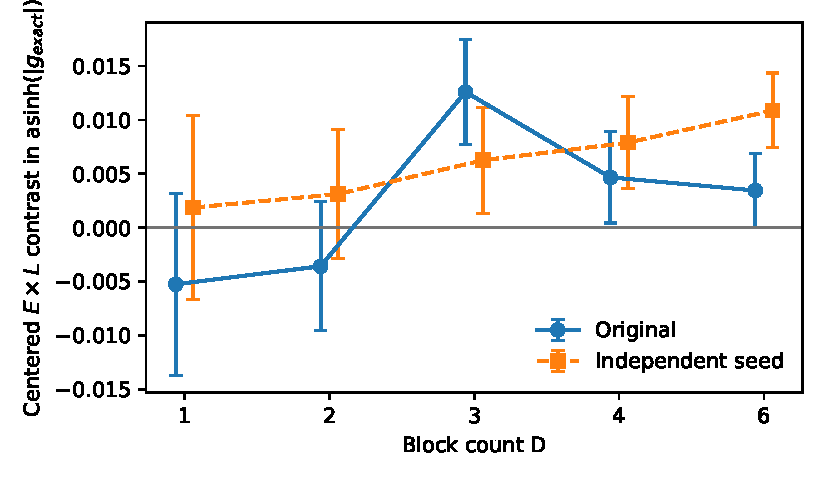
\includegraphics[width=0.78\textwidth]{figures/fig13_h1_depth.pdf}
\caption{Post-primary centered $E\times L$ exact-gradient contrasts by block count in the original and independent-seed datasets. Points show covariance-aware mixed-model contrasts and bars show unadjusted Wald 95\% intervals. Shape and line style distinguish datasets; the horizontal reference is zero. The display does not posit a monotonic depth law.}
\label{fig:h1-depth}
\end{figure*}

\begin{figure}[t]
\centering
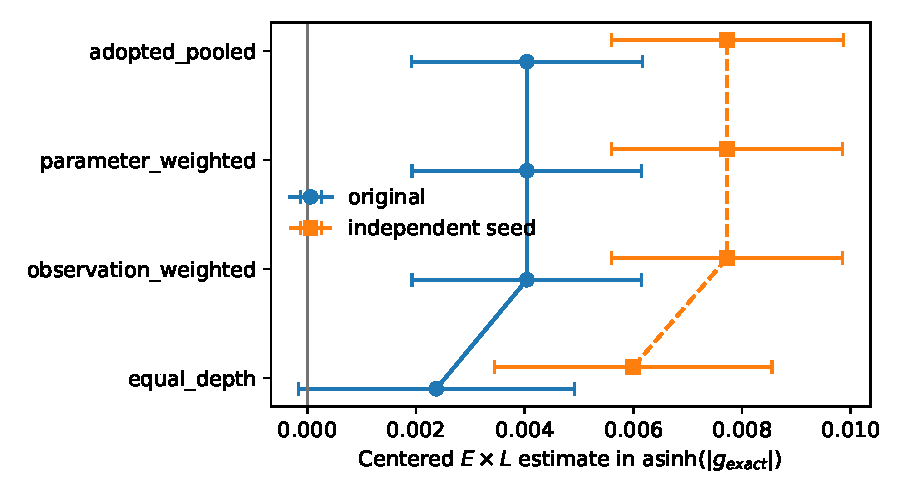
\includegraphics[width=\columnwidth]{figures/fig14_h1_weighting.pdf}
\caption{Post-primary H1 weighting summaries. Equal-depth and observation/matched-parameter weighting answer different questions; the adopted pooled estimate is shown separately. Bars are Wald 95\% intervals, and zero is the reference. Statistical significance is not a criterion for choosing a weighting.}
\label{fig:h1-weighting}
\end{figure}

\begin{figure}[t]
\centering
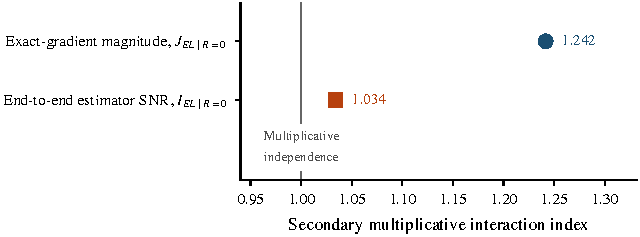
\includegraphics[width=\columnwidth]{figures/fig0_el_primary.pdf}
\caption{Descriptive multiplicative $E\times L$ indices conditional on $R=0$. $I_{EL\mid R=0}$ summarizes end-to-end estimator SNR and $J_{EL\mid R=0}$ exact-gradient magnitude; neither is a centered mixed-model coefficient. The line at one is the multiplicative no-interaction reference.}
\label{fig:el-primary}
\end{figure}

\subsection{Finite-shot interaction (H2)}\label{sec:h2-result}

Among positive-variance-eligible end-to-end cells, the corrected centered $E\times L$ coefficient was $0.014338$ (SE $0.005145$, Wald 95\% CI $[0.004255,0.024422]$, raw $p=0.005321$, Holm $p=0.015963$). The model-based Wald/Holm rule rejects H2. Its 443-completed-fit nested-bootstrap interval, $[-0.016638,0.043563]$, includes zero. H2 is therefore procedure-sensitive and is not independently corroborated by the nested bootstrap.

\subsection{Residual-related interactions (H3 and H4)}\label{sec:residual-results}

The corrected centered end-to-end $E\times R$ coefficient averaged across $L$ was $-0.011615$ (SE $0.005144$, Wald 95\% CI $[-0.021697,-0.001534]$, raw $p=0.023937$, Holm $p=0.047875$). The model-based rule rejects H3, but its 443-completed-fit percentile interval $[-0.030943,0.010259]$ includes zero. Matched $R=0$ and $R=1$ gradients are exactly equal at $D=1$ and $D=2$, as required by the inactive shortcut; this structural check passed exactly.

Post-primary end-to-end contrasts explain the averaging: at $L=0$ the estimate was $-0.000958$ (CI $[-0.015251,0.013336]$, $p=0.896$), whereas at $L=1$ it was $-0.022273$ (CI $[-0.036493,-0.008052]$, $p=0.00214$). All corresponding 443-fit bootstrap intervals include zero. At active depths $D\in\{3,4,6\}$, the L-averaged estimate was $-0.014788$ (CI $[-0.024480,-0.005095]$); $L=0$ remained near zero and $L=1$ was $-0.027449$. Depth-specific averages were $0.006642$, $0.000696$, $-0.026492$, $-0.011553$, and $-0.011255$ at $D=1,2,3,4,6$. Neither model-based ($p=0.545$) nor cluster-robust ($p=0.721$) moderation rejected. Conditional mode reversed direction ($0.006978$, CI $[-0.004745,0.018701]$). Thus H3 is a model-dependent directional signal, objective-specific under end-to-end mode, not a robust or confirmed residual interaction.

The corrected centered $L\times R\times$depth coefficient was $-0.010179$ (SE $0.005362$, Wald 95\% CI $[-0.020688,0.000331]$, raw and Holm $p=0.057658$). Its 443-fit percentile interval was $[-0.026975,0.006403]$. H4 is not rejected and remains unresolved; this is not evidence of absence.

\begin{table*}[t]
\centering
\footnotesize
\begin{tabularx}{\textwidth}{@{}l p{0.13\textwidth} r l r l >{\raggedright\arraybackslash}X@{}}
\toprule
Hyp. & Estimand & Estimate & Wald 95\% CI & Holm $p$ & Bootstrap 95\% CI & Evidence summary \\
\midrule
H1 & $E_cL_c$, exact
   & 0.004043
   & \mbox{$[0.001924,\,0.006162]$}
   & 0.000739
   & \mbox{$[0.000473,\,0.007535]$}
   & Both methods \\
H2 & $E_cL_c$, end-to-end
   & 0.014338
   & \mbox{$[0.004255,\,0.024422]$}
   & 0.015963
   & \mbox{$[-0.016638,\,0.043563]$}
   & Wald only \\
H3 & $E_cR_c$, end-to-end
   & -0.011615
   & \mbox{$[-0.021697,\,-0.001534]$}
   & 0.047875
   & \mbox{$[-0.030943,\,0.010259]$}
   & Wald only \\
H4 & $L_cR_c\times$depth
   & -0.010179
   & \mbox{$[-0.020688,\,0.000331]$}
   & 0.057658
   & \mbox{$[-0.026975,\,0.006403]$}
   & Neither \\
\bottomrule
\end{tabularx}
\caption{Corrected centered H1--H4 family. Wald intervals and Holm-adjusted $p$-values follow the primary model-based decision rule; the Bootstrap 95\% CI column gives initialization-cluster percentile intervals. ``Both methods'' means that the Wald and bootstrap intervals exclude zero; ``Wald only'' means that the Wald/Holm rule rejects while the bootstrap interval includes zero; and ``Neither'' means that the Wald/Holm rule does not reject and the bootstrap interval includes zero. H1 used 2,000 completed bootstrap fits with zero failures, whereas H2--H4 used 443 completed nested-bootstrap fits. Bootstrap iterations are distinct from the 50 independent initialization clusters.}
\label{tab:confirmatory-summary}
\end{table*}

\begin{figure}[t]
\centering
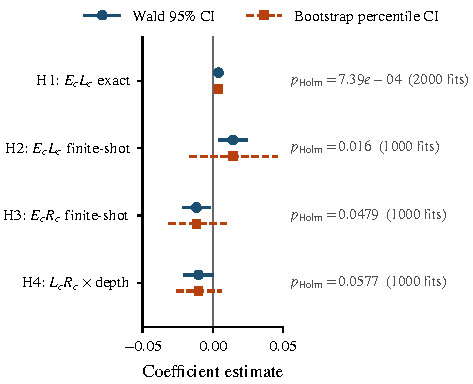
\includegraphics[width=\columnwidth]{figures/fig1_confirmatory_forest.pdf}
\caption{Corrected primary Wald 95\% intervals and initialization-cluster percentile bootstrap intervals for H1--H4, with a zero reference. H1 used 2,000 completed bootstrap fits; H2--H4 used 443. Marker shape and line style distinguish interval types without reliance on color.}
\label{fig:confirmatory-forest}
\end{figure}

\subsection{Conditional multiplicative indices}

For the original data, $J_{EL\mid R=0}=1.241760$ (bootstrap median $1.238674$, 95\% percentile CI $[1.082210,1.414864]$). At $R=1$, $J_{EL\mid R=1}=1.126633$ (median $1.124329$, CI $[0.991331,1.285152]$), and this interval includes one. New-seed values were $1.163219$ at $R=0$ (median $1.160949$, CI $[1.007100,1.352596]$) and $1.242137$ at $R=1$ (median $1.238157$, CI $[1.049874,1.449258]$). Each bootstrap completed 2,000 iterations with zero failures. These weighting-dependent ratios are descriptive and conditional on $R$; they are not percent improvements and do not measure optimization.

\subsection{Prepared-state metrics and implemented resources}

All bounds, uniqueness, and fidelity--infidelity complementarity checks passed for 4,000 unique terminal-block prepared states at initialization. Cell mean fidelity ranged approximately $0.0338$--$0.0817$ in the original data and $0.0322$--$0.0962$ in the independent-seed data; normalized prepared-state energy means ranged $0.4631$--$0.5529$ and $0.4561$--$0.5537$, respectively. The ranges overlap strongly and show no conspicuous seed-unstable separation descriptively. They do not demonstrate training success or a causal relationship between gradient magnitude and task quality.

All 320 resource-design rows conserve nominal implemented $B$, with no negative allocations or zero-shot production jobs. All 1,833 zero-variance cells joined to complete resource records. At $D=6$, the extremes are 48 jobs for conditional/global and 61 for end-to-end/local, a 27.08\% increase. This is a simulator job-count comparison, not a matched physical-resource or wall-clock claim.

\subsection{Implementation checks}\label{sec:results-robustness}

Black-box finite differences checked 224 quantum-parameter derivatives across 16 cases at $D=1$ and $D=6$, configurations 1, 2, 3, and 5, and steps $10^{-3},10^{-4},10^{-5}$. At $10^{-5}$, the maximum relative error was $1.27\times10^{-5}$ overall and $9.77\times10^{-7}$ among 214 gradients with magnitude at least $10^{-5}$; four near-zero gradients exceeded the relative tolerance but retained six-significant-figure absolute agreement, with no sign or order-of-magnitude failures. Centered and direct models were verified as exact reparameterizations, estimator modes were guarded against pooling, and frozen outputs passed deterministic regeneration and manifest-integrity tests. The adopted H2--H4 fit converged with L-BFGS, was nonsingular, emitted one boundary warning, and agreed with BFGS to 8--9 significant figures; residual heteroscedasticity and heavy tails remain covariance caveats. Online Resource 1 reports complete diagnostics.

\section{Discussion}

\subsection{Principal findings}

H1 provides the strongest cross-procedure evidence. Its positive centered exact-gradient direction appears in both seed sets and both initialization-cluster bootstrap intervals exclude zero. Its magnitude and depth profile nevertheless remain uncertain: the seed-set point estimates differ, the original equal-depth interval includes zero while its observation-weighted interval does not, and the original moderation conclusion depends on covariance estimator.

H2 and H3 require a different interpretation. Both meet the primary model-based Wald/Holm rejection rule, yet their nested-bootstrap intervals include zero. H2 is additionally conditional on objective-linked positive-variance eligibility. H3's end-to-end direction is concentrated in the energy-objective condition, reverses under conditional mode, and is not supported by cluster-robust depth moderation. H4 is not rejected and remains unresolved rather than proved absent. Post-primary analyses therefore indicate that H1's pooled positive direction is reproducible across seed sets, but its magnitude and depth profile are uncertain; H2 and H3 remain procedure-sensitive because their Wald/Holm rejections are not corroborated by the corresponding nested-bootstrap intervals.

Conditional $J$ ratios provide descriptive multiplicative summaries, with positive above-reference patterns in several dataset--residual combinations. They are weighting-dependent, conditional on $R$, and not algebraic equivalents of centered mixed-model coefficients. Prepared-state metrics likewise describe initialization states only; they neither demonstrate training success nor establish that larger initial gradients causally improve energy or fidelity. Resource accounting applies to the implemented simulator protocol: total $B$ is conserved, but job counts and shots per job differ, and no physical-resource or hardware-cost equality follows.

\subsection{Interpretation and relation to prior work}

Local objectives can improve gradient scaling under specified circuit-depth assumptions, while excessive random entanglement can suppress gradients \cite{cerezo2021costfunction,ortizmarrero2021entanglement,patti2021entanglement}. The present result connects these observations statistically: in this four-qubit reset-based architecture, the modeled objective contrast is larger under the restricted CNOT schedule than expected from the two marginal effects on the transformed response scale. This non-additivity is compatible with theoretical accounts that treat architecture, state structure, and observable support as coupled determinants of loss concentration \cite{ragone2024lie}, but it neither identifies a physical mechanism nor tests asymptotic barren-plateau scaling.

The $L$ factor also changes more than measurement locality. Normalized TFIM energy and global infidelity differ in spectral weighting, observable decomposition, circuit count, and landscape geometry. Likewise, the $E$ factor is one specific four-CNOT schedule and the $R$ factor is one fixed-gain shortcut between reset blocks. The observed coefficients should therefore be interpreted as interactions among these implemented contrasts, not universal laws about low entanglement, local costs, or residual quantum networks.

The results concern matched initial parameter points rather than complete optimization trajectories. A resolvable initial gradient is neither necessary nor sufficient for convergence, and residual architectures evaluated over full training trajectories address a different estimand \cite{anschuetz2022traps,grant2019identity,skolik2021layerwise,kashif2024resqnets}. The unstable residual-interaction evidence here does not contradict optimization results in other architectures.

\subsection{Implications for QML evaluation}

The study shows why gradient-resolvability interventions should not be evaluated only one at a time. A factorial design can reveal pairwise non-additivity and moderation without implying that a fully combined configuration is universally preferable. Future benchmarks should test both whether interventions interact and whether those interactions vary with architecture-size variables.

Finite-shot metrics also require operational definitions that are treated as part of the experiment. Matching total shots does not match per-circuit precision; re-estimating intermediate features changes bias and sign reliability; and plug-in ratios can generate factor-dependent eligibility when estimated variance is zero. Eligibility rules, estimator modes, seed derivation, and regression guards should be specified and tested as carefully as the statistical formula itself.

\subsection{Limitations and priorities for follow-up}\label{sec:limitations}

The experiment covers four qubits, one open-boundary TFIM task, one reset-per-block architecture, one implementation of each intervention, one initialization family, and 50 top-level initialization clusters per dataset where applicable. Exact-state and abstract shot simulation omit hardware noise, readout and calibration models, and wall-clock behavior. There are no optimization trajectories; task metrics are terminal-block prepared-state quantities at initialization only.

Finite-replicate zero-variance selection is tied to $L$. Increasing parameter count with depth induces observation/parameter weighting, and some depth conclusions are covariance-sensitive. H2 and H3 disagree across inference procedures, while H3 also disagrees across estimator modes. Conditional $J$ quantities are weighting-dependent descriptive summaries. The reset-per-block reading and inaccessible full protocol text remain provenance limitations for the original architecture and factor-coding specification. No matched physical-resource claim is available because circuits, jobs, shots per circuit, gates, calibration, readout, noise, and time were not jointly matched.

Follow-up work would require prospectively specified additional datasets, continuous-state architectural controls, optimization trajectories, and hardware-noise experiments; none is inferred from the present initialization analysis.

\section{Conclusion}\label{sec:conclusion}

The strongest cross-procedure evidence concerns H1. The positive centered $E\times L$ exact-gradient interaction was retained in a new-seed dataset, although its magnitude, depth profile, covariance dependence, and weighting dependence remain uncertain. H2 and H3 satisfy the model-based Wald/Holm rule but have bootstrap intervals spanning zero, while H4 remains unresolved. These results support factorial and measurement-aware benchmarking of gradient usability, but do not establish optimization, hardware, or resource advantage.

\backmatter

\section*{Statements and Declarations}

\bmhead{Funding} No external funding was received.

\bmhead{Competing interests} The author declares no financial or non-financial competing interests.

\bmhead{Ethics approval} Not applicable. This study used computational simulations and did not involve human participants, human data, animals, or biological materials.

\bmhead{Consent to participate} Not applicable.

\bmhead{Consent for publication} Not applicable.

\bmhead{Author contributions} Brandon Shen conceived the study, implemented the simulation and analysis pipeline, conducted the experiments and verification analyses, interpreted the results, prepared the figures, and wrote and revised the manuscript.

% Before submission, mint a versioned archival DOI (for example via Zenodo) and add it here if available.
\bmhead{Data availability} The machine-readable numerical source is \texttt{results/final\_submission\_v1/manifest.json}. The immutable numerical-results freeze is \nolinkurl{submission-numerical-results-freeze-v1}. The finalized manuscript-facing repository snapshot is the release \href{https://github.com/Brandon-Shen/few-qubit-qnn-snr/tree/sncs-submission-v2}{\texttt{sncs-submission-v2}}. Files under \path{results/superseded/}, \path{results/superseded_pooled/}, and other explicitly superseded directories are historical material and must not be read as current primary conclusions. \texttt{MANUSCRIPT\_COMMIT.txt} records the exact substantive commit against which the manuscript sources, numerical values, tables, figures, and documentation were finalized.

\bmhead{Code availability} The final immutable manuscript, code, documentation, verification scripts, and submission-facing repository state are available in the \href{https://github.com/Brandon-Shen/few-qubit-qnn-snr/tree/sncs-submission-v2}{\texttt{sncs-submission-v2}} release. This release is distinct from the numerical-results freeze identified above. The repository contains the simulation and gradient code, mixed-model and multiplicity analyses, bootstrap implementations, robustness analyses, figure scripts, and regression tests; \texttt{MANUSCRIPT\_COMMIT.txt} identifies the finalized substantive repository state.

\bmhead{Materials availability} Not applicable.

\bmhead{Software and reproducibility information} Analyses used Python 3.12.10, PennyLane 0.45.1, pandas 3.0.3, NumPy 2.5.1, statsmodels 0.14.6, SciPy 1.18.0, Matplotlib 3.11.0, PyArrow 25.0.0, and PyYAML 6.0.3. Random seeds are derived deterministically from a root seed, named stream, and cell identifiers via SHA-256. Model convergence, optimizer agreement, warnings, frozen inputs, and script-level provenance are documented in Online Resource 1 and the repository; no blanket convergence claim is inferred beyond those frozen records.

\bmhead{Supplementary information} Online Resource 1 contains additional estimator-eligibility analyses, model and influence diagnostics, the documented estimator-mode correction, bootstrap and depth-sensitivity results, and a reproducibility index. The supplementary file is provided as \texttt{ESM\_1.pdf}.

\bibliography{references}

\end{document}
